\documentclass[12pt]{article}
\usepackage{setspace}
\setstretch{1}
\usepackage{amsmath,amssymb, amsthm}
\usepackage{graphicx}
\usepackage{bm}
\usepackage[hang, flushmargin]{footmisc}
\usepackage[colorlinks=true]{hyperref}
\usepackage[nameinlink]{cleveref}
\usepackage{footnotebackref}
\usepackage{url}
\usepackage{listings}
\usepackage[most]{tcolorbox}
\usepackage{inconsolata}
\usepackage[papersize={8.5in,11in}, margin=1in]{geometry}
\usepackage{float}
\usepackage{caption}
\usepackage{esint}
\usepackage{url}
\usepackage{enumitem}
\usepackage{subfig}
\usepackage{wasysym}
\newcommand{\ilc}{\texttt}
\usepackage{etoolbox}
\usepackage{algorithm}
% \usepackage{algorithmic}
\usepackage[noend]{algpseudocode}
\usepackage{tikz}
\usepackage{listings}
\usepackage{color}
\usetikzlibrary{matrix,positioning,arrows.meta,arrows}
\patchcmd{\thebibliography}{\section*{\refname}}{}{}{}



\definecolor{dkgreen}{rgb}{0,0.6,0}
\definecolor{gray}{rgb}{0.5,0.5,0.5}
\definecolor{mauve}{rgb}{0.58,0,0.82}

\lstset{frame=tb,
  language=Python,
  aboveskip=3mm,
  belowskip=3mm,
  showstringspaces=false,
  columns=flexible,
  basicstyle={\small\ttfamily},
  numbers=none,
  numberstyle=\tiny\color{gray},
  keywordstyle=\color{blue},
  commentstyle=\color{dkgreen},
  stringstyle=\color{mauve},
  breaklines=true,
  breakatwhitespace=true,
  tabsize=3
}

\begin{document}

\title{\textbf{CSDS 313: Assignment 3}}

\author{Shaochen (Henry) ZHONG, \ilc{sxz517} \\Ningjia HUANG, \ilc{nxh239}}
\date{Due and submitted on 11/23/2020 \\ Issued by Dr. Koyut{\"u}rk}
\maketitle

\section*{Problem 1}


\subsection*{(a)}
Select the significance level $\alpha$ = 0.05. \\

\noindent\textbf{Mutual Information}: \\
Let column 1 be random variable $X$, column 2 be random variable $Y$.
\begin{center}
    \begin{tabular}{ | c | c | c | }
        \hline
        Value of $X$ & $p$ & $-plog_{2}p$ \\
        \hline
        $X = 0$ & 0.7487437185929648 & 0.5006955856203327 \\
        \hline
        $X = 1$ & 0.25125628140703515 & 0.31256763272432964 \\
        \hline
        Total & $1.0$ & 0.8132632183446623 \\
        \hline
        \end{tabular}
\end{center}

\begin{center}
  \begin{tabular}{ | c | c | c | }
      \hline
      Value of $Y$ & $p$ & $-plog_{2}p$ \\
      \hline
      $Y = 0$ & 0.8944723618090452 & 0.14391272233543062 \\
      \hline
      $Y = 1$ & 0.10552763819095477 & 0.34236407614604353 \\
      \hline
      Total & $1.0$ & 0.48627679848147415 \\
      \hline
      \end{tabular}
\end{center}

\begin{center}
  \begin{tabular}{ | c | c | c | }
      \hline
      Value of $X,Y$ & $p$ & $-plog_{2}p$ \\
      \hline
      $X = 0, Y = 0$ & 0.6432160804020101 & 0.40948719311350273 \\
      \hline
      $X = 1, Y = 0$ & 0.25125628140703515 & 0.5006955856203327 \\
      \hline
      $X = 0, Y = 1$ & 0.10552763819095477 & 0.34236407614604353 \\
      \hline
      $X = 1, Y = 1$ & 0.0 & 0.0 \\
      \hline
      Total & $1.0$ & 1.252546854879879 \\
      \hline
      \end{tabular}
\end{center}
$MI = E(X) + E(Y) - E(X,Y) = 0.8132632183446623 + 0.48627679848147415 - 1.252546854879879 = 0.046993161946257356$ \\ \\
\textbf{The output we generated from $200$ permutation tests are:} \\ \\
num of permutation:  0 , mutual information: $0.03414403902960417$ \\
num of permutation:  1 , mutual information: $0.04335451902085774$ \\
num of permutation:  2 , mutual information: $0.0683942335508787$ \\
$\dots$ \\
num of permutation:  198 , mutual information: $0.04044540484946402$ \\
num of permutation:  199 , mutual information: $0.04044540484946402$ \\
num of more significant value:  16 \\ \\
Therefore, the $p-value$ is $\frac{16+1}{200+1} = 0.0845771144$, which is larger than the significance level $\alpha$ we chose(0.05)
, proving the null hypothesis to be true. However, the p-value is only about $3\%$ higher than the significance level we choose, which
cannot serve as a strong evidence to prove the hypothesis. This may due to the small size of permutation tests we chose. If we perform
more permutation tests, the p-value is likely to go down. \\

\noindent\textbf{Jaccard Index: } \\
Select the significance level $\alpha = 0.05$. \\
The jaccard index for the dataset is calculated by: $\frac{x_1y_1}{x_0y_1 + x_1y_0 + x_1y_1} = 0.0$ \\ \\
\textbf{The result we generated from 200 permutation tests are: } \\ \\
Jaccard Index for data:  0.0 \\
Jaccard Index for data:  0.0 \\
$\dots$ \\
Jaccard Index for data:  0.0 \\
Jaccard Index for data:  0.0 \\
num of more significant value:  0 \\ \\
Therefore, the $p-value$ is $\frac{0+1}{200+1} = 0.0049751$, which is smaller than the significance level $\alpha$ we chose(0.05). Therefore, we can reject the null hypothesis, which is there is no association between these two attributes.
It seems the p-value is pretty close to the significance level we chose, which may lead to a relatively weak association, but it is actually due to the number of permutation we performed. If we perform $1,000$ permutations instead of $200$, the
p-value would decrease significantly. Therefore, we can safely conclude that these two variables are statistically significantly associated.
The result for jaccard index is straight-forward: it indicates that in all 199 paris of individuals, there is no individual who has
1s for both X and Y genomic variants. \\

\noindent\textbf{Pearson's chi squared $X^2$: } \\
Select the significance level $\alpha = 0.05$.
\begin{center}
  \begin{tabular}{ | c | c | c | c |}
      \hline
       & $Y = 0$ & $Y = 1$ & Total\\
      \hline
      $X = 0$ & 128  & 21 & 149 \\
      \hline
      $X = 1$ & 50 & 0 & 50 \\
      \hline
      Total & 178 & 21 & 199 \\
      \hline
  \end{tabular}
\end{center}
The chi-square for the dataset is: $7.87836513083478$. \\
According to the problem, Pearson's chi-squared follows a well-studied distribution called chi-squared distribution. Therefore,
we can use the calculated value of chi-squared as well as the degree of freedom to estimate the $p-value$. As shown above, the contingency
table contains two rows and two columns, which gives us a degree of freedom $df = (r-1)(c-1) = (2-1)(2-1) = 1$.
By using the online link(\href{https://www.socscistatistics.com/pvalues/chidistribution.aspx}{P Value from Chi Square Calculator}),
we get the p-value of ``there is no association between these two genomic variants'' to be $0.005003$. As we select the significance level $\alpha$
to be $0.05$, it provides a suggestion that these two hypothesis may not be significantly associated. However, note that the p-value is only $0.0000003$
higher than the significance level we chose, which is not strong enough to prove the correctness of the null hypothesis. This may due to the limited sample
size or the small number of permutation tests we've conducted. \\

\noindent Overall, these three statistics agree with each other and suggest these two attributes are significantly associated. Although the chi-square statistic proves
the null hypothesis, it is only $0.0000003$ higher than the null hypothesis and cannot be a strong evidence to prove the null hypothesis. Jaccard's index proves these two
variables are significantly associated, but since the p-value is not significantly smaller than the significance level, it is not a strong proof. The mutual information Is
a little bit higher than the significance level we chose, which may be due to the small permutation size I chose.

\subsection*{(b)}
\subsubsection*{Mutual Information: }
Tuple( A , B ): 0.054093383055560995  Tuple( A , C ): 0.3770318235987944 \\
Tuple( A , D ): 0.7098907780024963  Tuple( A , E ): 0.05674106401270551 \\
Tuple( A , F ): 0.19129241546358777  Tuple( A , G ): 0.7370862500524509 \\
Tuple( A , H ): 0.557383937289774  Tuple( A , I ): 0.43424968973657685 \\
\dots \\
Tuple( L , O ): 0.019314328814340476  Tuple( M , N ): 0.07906298064106565 \\
Tuple( M , O ): 0.03806565500381831  Tuple( N , O ):  9.990567284057228e-05 \\

\noindent Select the significance level $\alpha = 0.05$. By using Benjamini-Hochberg Procedure to adjust the false discovery rate,
we got 96 out of 105 hypothesis that are less than the significance level(α= 0.05).


\begin{center}
  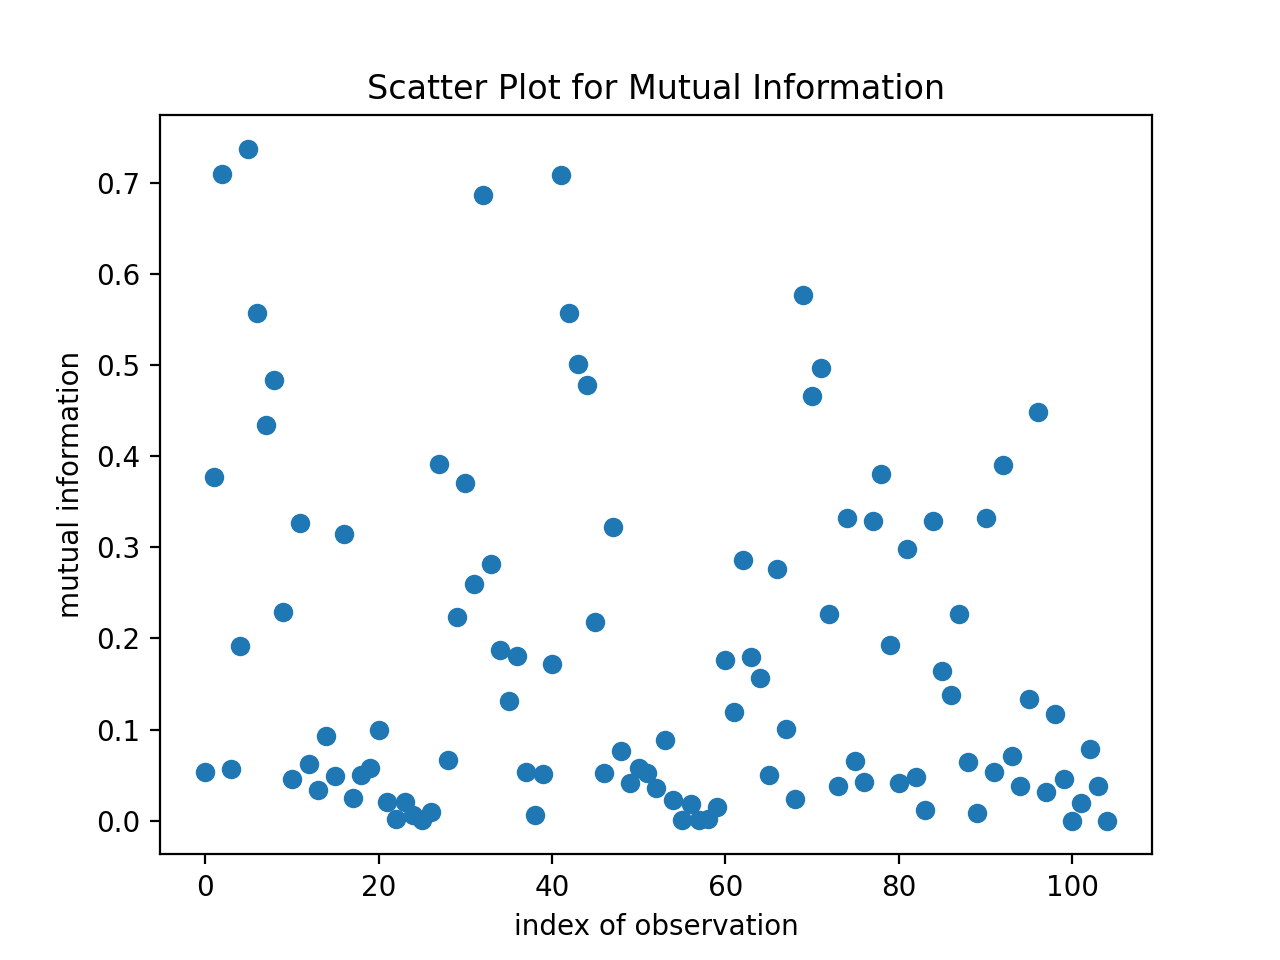
\includegraphics[width=0.5\linewidth]{{fig/p1b_mutual_information.png}}
\end{center}


\begin{figure}[H]
    \centering
    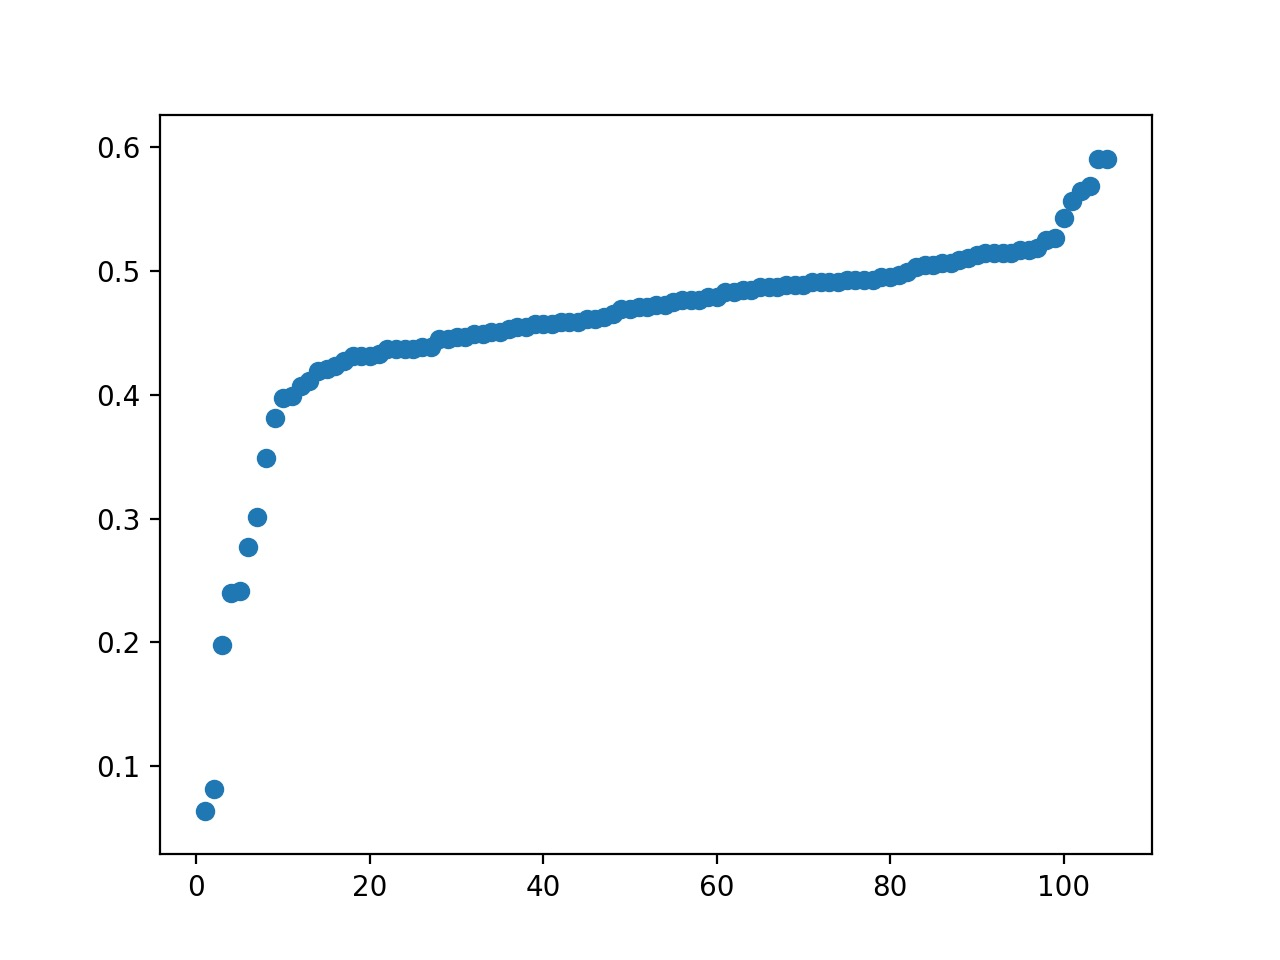
\includegraphics[width=0.5\linewidth]{{fig/fig_1b_alt.jpg}}
    \caption{Sorted P-values list for MI}
\end{figure}

\subsubsection*{Jaccard Index: }
Select the significance level $\alpha = 0.05$.
Tuple( A B ), jaccard index:  0.0 \\
Tuple( A C ), jaccard index:  0.6410256410256411 \\
Tuple( A D ), jaccard index:  0.9259259259259259 \\
\dots \\
Tuple( M N ), jaccard index:  0.1 \\
Tuple( M O ), jaccard index:  0.24752475247524752 \\
Tuple( N O ), jaccard index:  0.13636363636363635 \\

\begin{center}
  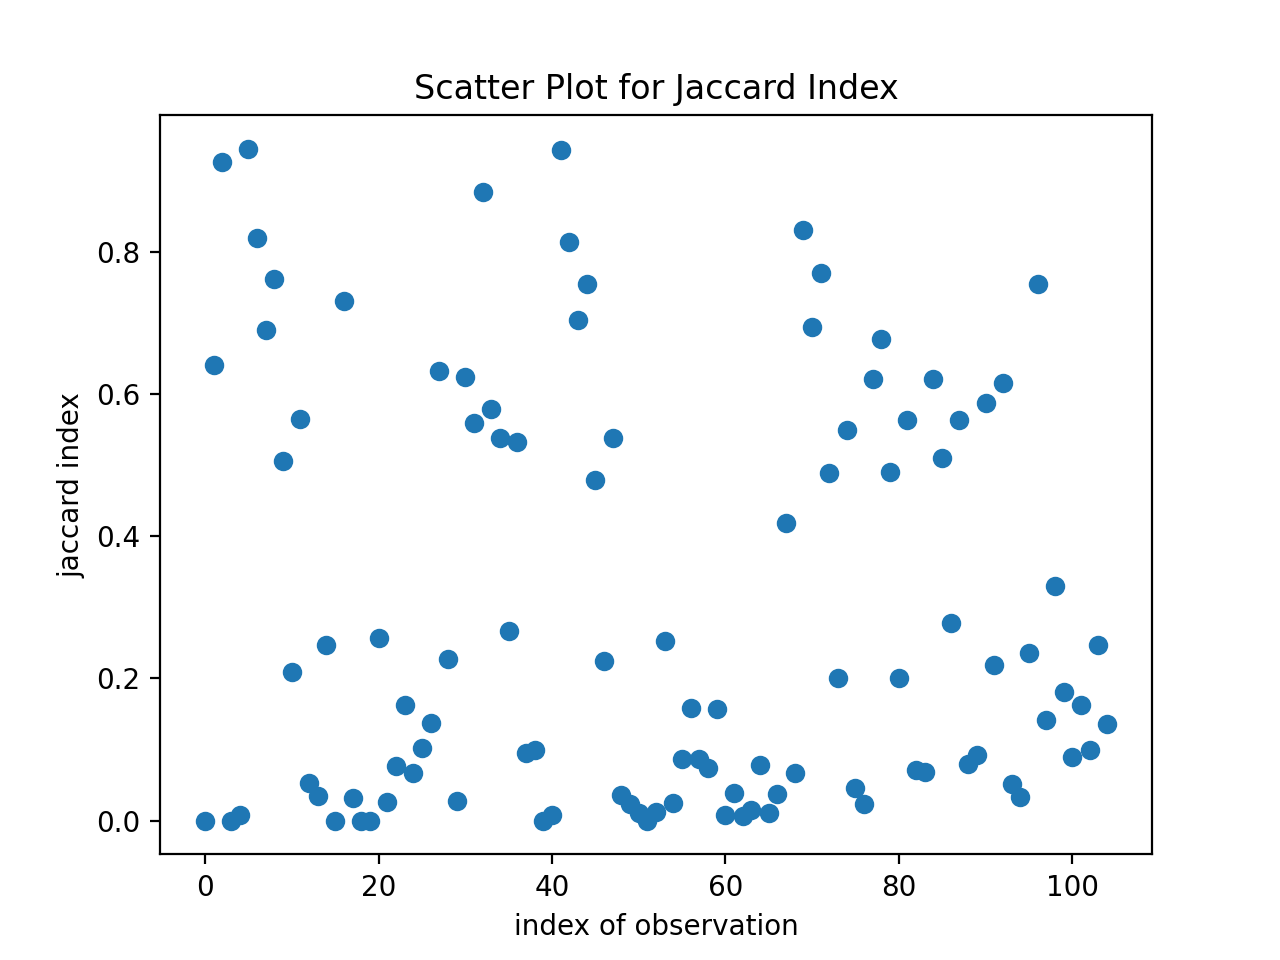
\includegraphics[width=0.5\linewidth]{{fig/p1b_jaccard_index.png}}
\end{center}

By conducting $N=500$ permutation tests with sample size $n=50$, we generated the distribution of p-value for Jaccard Index. The following graph shows the p-value distribution for Jaccard Index:

\begin{center}
  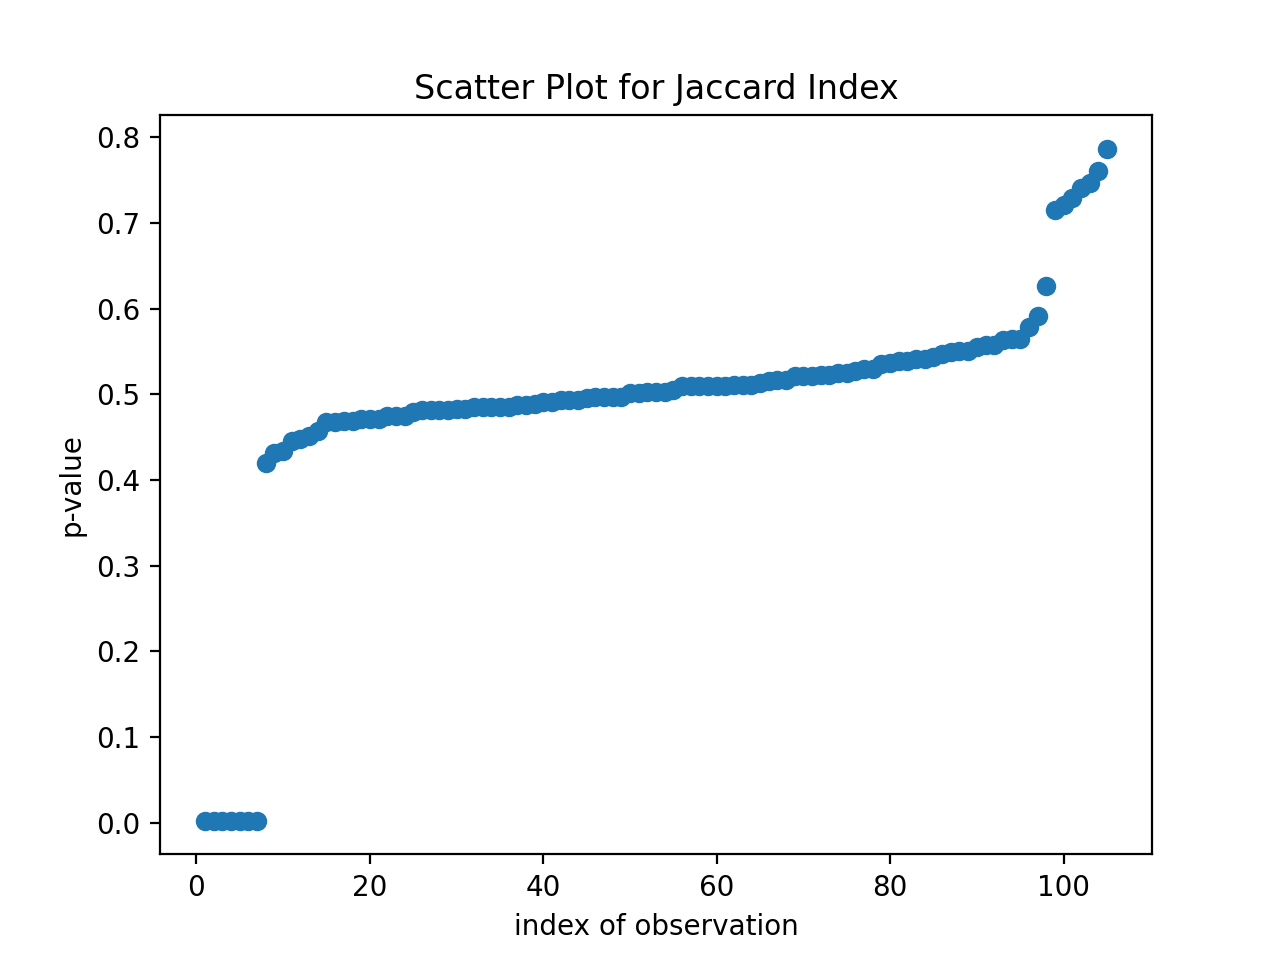
\includegraphics[width=0.5\linewidth]{{fig/p1b_jaccard_p-value.png}}
\end{center}

Without using Benjamini-Hochberg Procedure to adjust the false discovery rate, we got 17 out of 105 hypothesis that are less than the significance level($\alpha=0.05$).
By using BH Procedure, the largest p value that is smaller than the critical value we got is $0.001996007984031936$. Therefore, the adjusted total number of significant pairs we got is $105$.

\subsubsection*{Pearson's chi squared $X^2$:}
Tuple( A B ), chi squared =  9.2114552893045 \\
Tuple( A C ), chi squared =  97.40185818922372 \\
\dots \\
Tuple( M O ), chi squared =  10.406218057892048 \\
Tuple( N O ), chi squared =  0.027695410134060443 \\
The following graph shows the distribution of Pearson's chi-square:
\begin{center}
  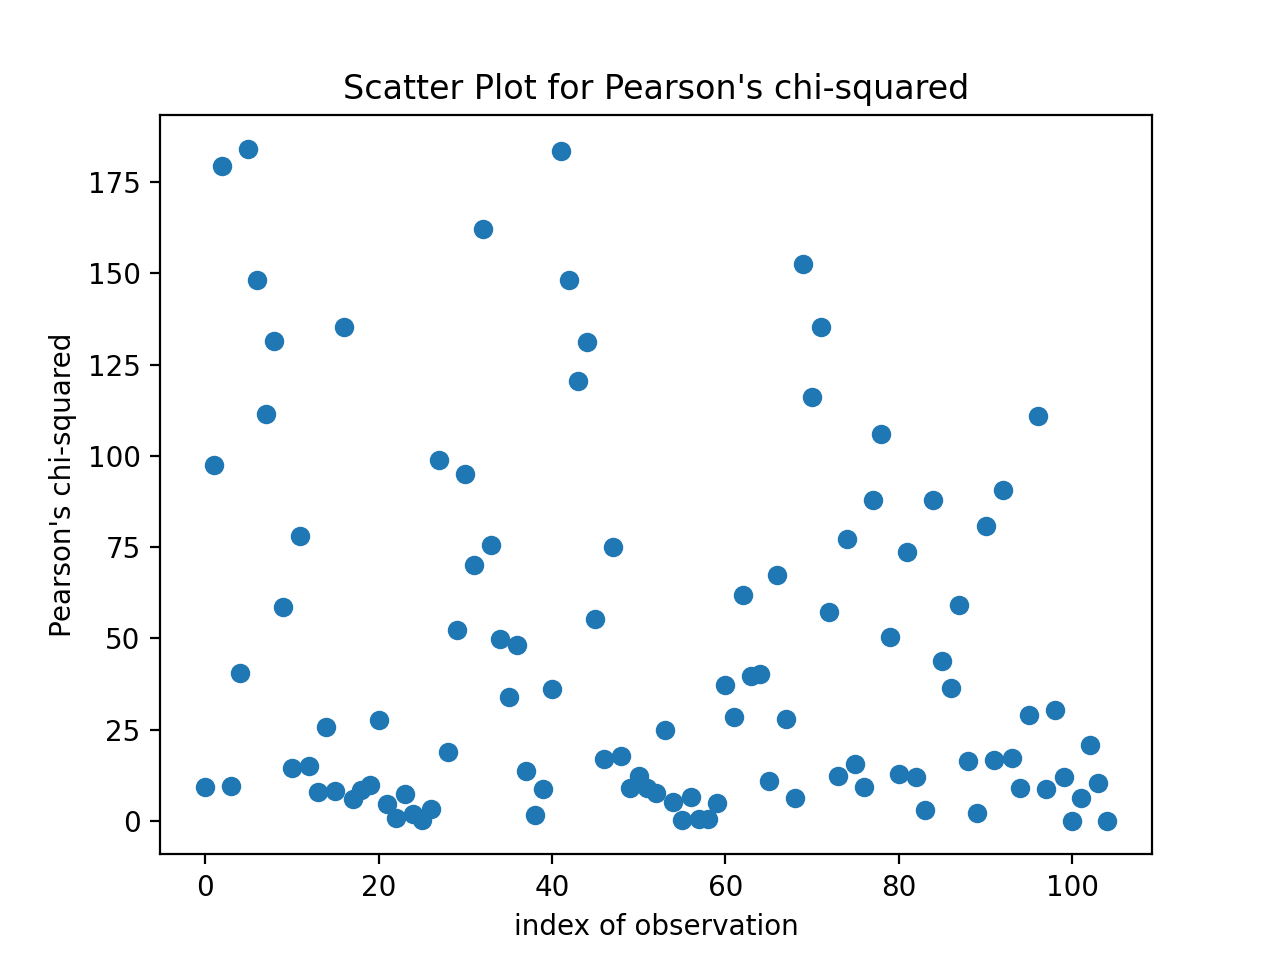
\includegraphics[width=0.5\linewidth]{{fig/p1b_chi_square.png}}
\end{center}
By conducting 500 permutation tests with sample size $n = 50$, we generated the distribution of p-value for Pearson's chi-squared. The following graph shows the p-value distribution for Pearson's chi-square:
\begin{center}
  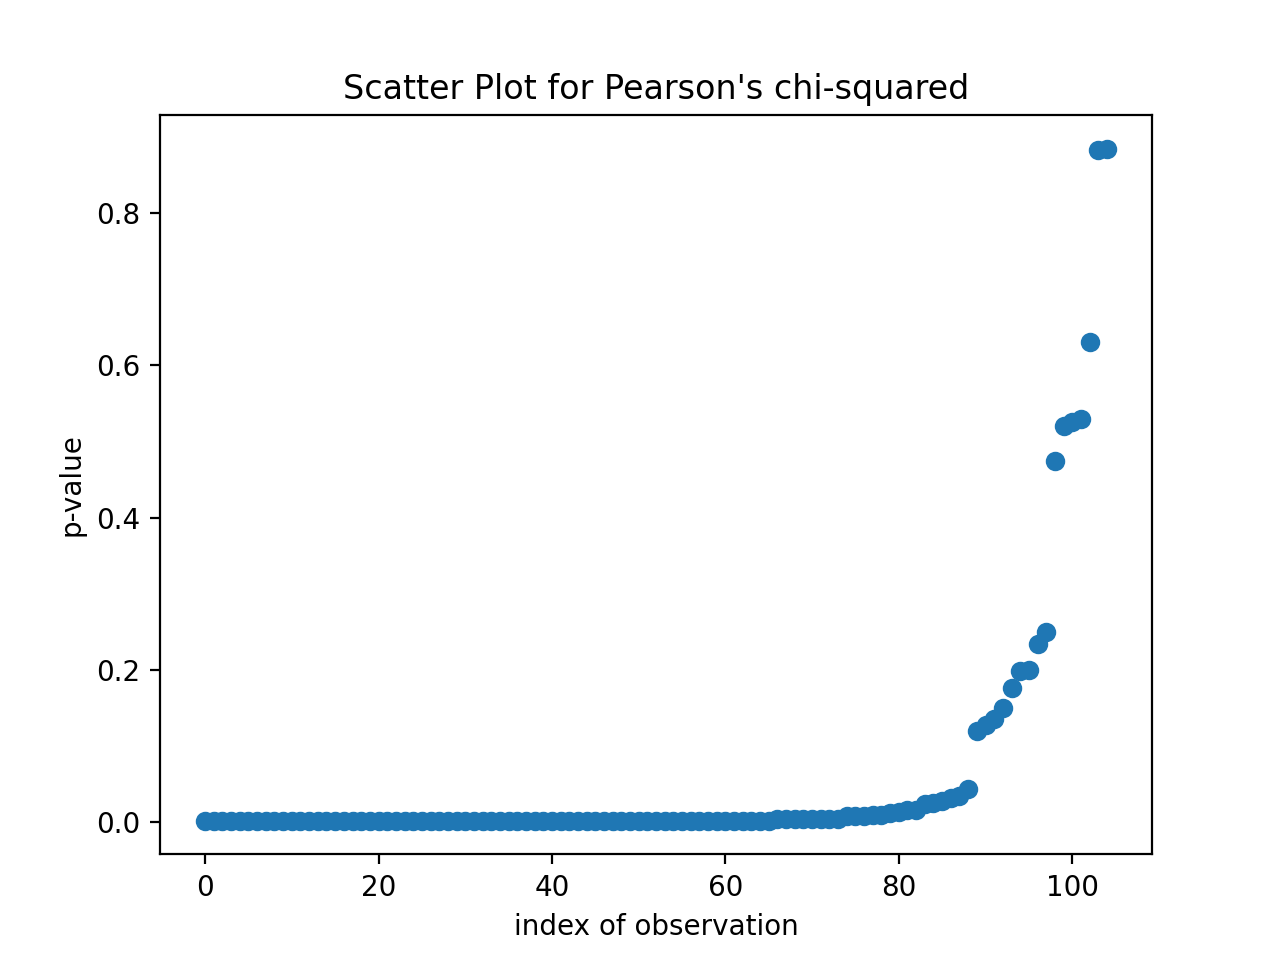
\includegraphics[width=0.5\linewidth]{{{fig/p1b_chi_square_p_value.png}}}
\end{center}
Without using Benjamini-Hochberg Procedure to adjust the false discovery rate, we got 17 out of 105 hypothesis that are less than the significance level($\alpha=0.05$).
By using BH Procedure, the largest p value that is smaller than the critical value we got is $0.038$. Therefore, the adjusted total number of significant pairs we got is $87$.

By first looking at the plots we made, we decide the more similar pair of statistics are mutual information and jaccard's index since they have similar distributions. Both of them reject the null hypothesis.
The following table shows the number of overlapping significant pairs:
\begin{center}
  \begin{tabular}{ | c | c | c | c |}
    \hline
     & $MI$ & $JI$ & $chi-square$\\
    \hline
    $MI$ & -  & 96 & 51 \\
    \hline
    $JI$ & 96 & - & 87\\
    \hline
    $chi-square$ & 51 & 87 & - \\
    \hline
\end{tabular}
\end{center}
As the table suggested, mutual information and jaccard's index have more overlapping pairs, which also proves that these two statistics are more similar to each other.
Personally speaking, I prefer to use chi-square statistic since it takes into account the sample size. For mutual information and jaccard index, the choice of sample size
for permutation test would be a problem since if the sample size is too small, the statistics cannot indicate the association between variables accurately. If we only consider
the Pearson's chi square, the result won't change since the adjusted p-value is $0.038$, which is still smaller than the significance level we chose.

\newpage

\section*{Problem 2}

Since all three subproblems of this problem are asking the same set of questions over different data set, W.L.O.G. here is the code used to produce result for \ilc{p2a.csv}.


\begin{lstlisting}
df_2a = pd.read_csv('assignment_3/data/p2a.csv', header=None)
print(f'p2a.csv Corr: {stats.pearsonr(df_2a[0], df_2a[1])[0]}; P-value: {stats.pearsonr(df_2a[0], df_2a[1])[1]}')
df_2a.plot.scatter(x = 0, y = 1)
plt.axis('square')
plt.title('p2a.csv')
\end{lstlisting}

\noindent Also, to make comparision easier, we opted to put all scatter plots of \ilc{variable 1} v. \ilc{variable 2} among all three dataset side-by-side together (please zoom in if you can't see it clearly, sorry).

\begin{figure}[H]
\minipage{0.32\textwidth}
  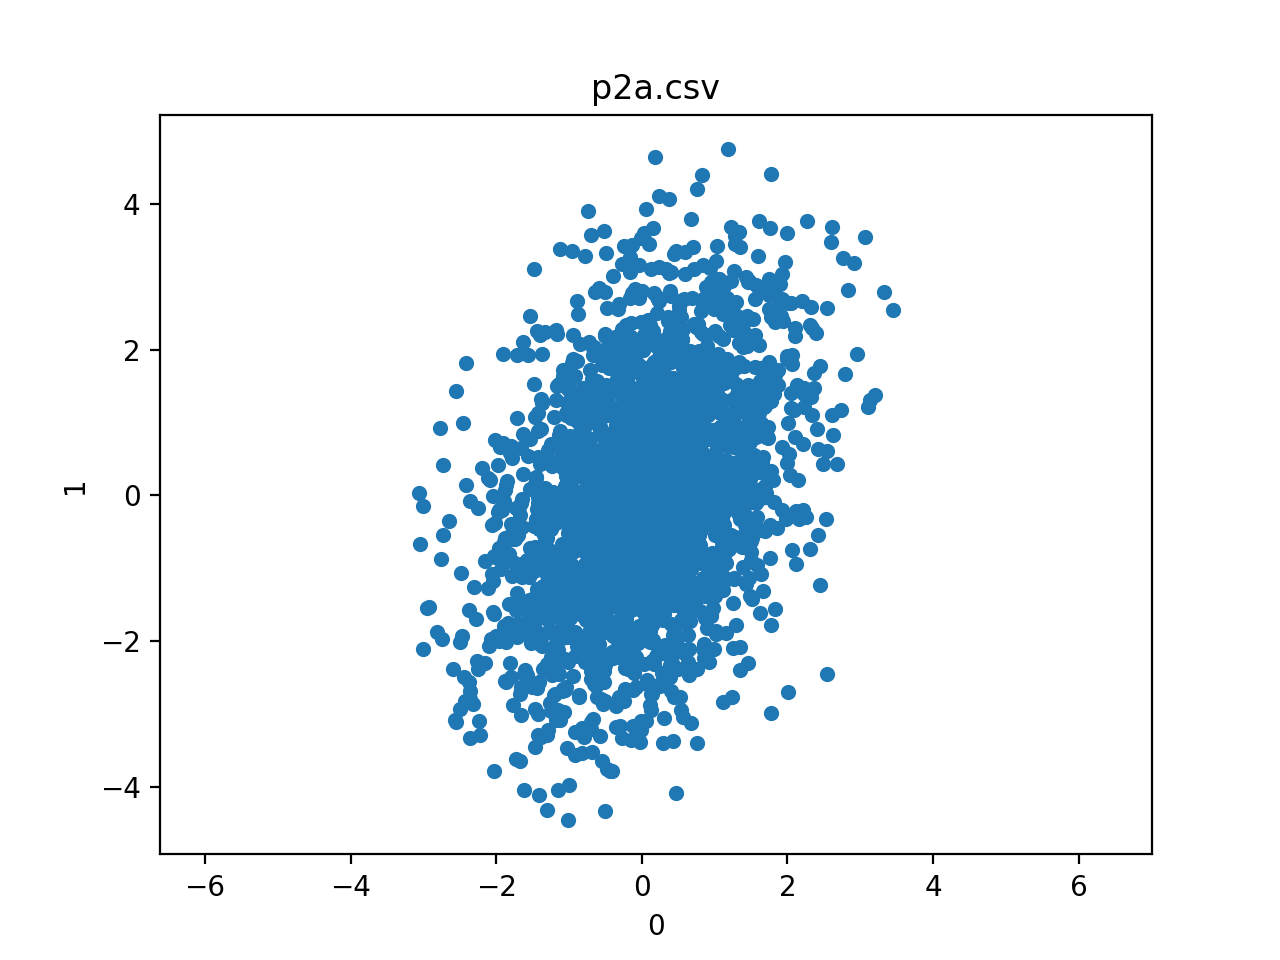
\includegraphics[width=\linewidth]{{fig/fig_p2a_1.png}}
\endminipage\hfill
\minipage{0.32\textwidth}
  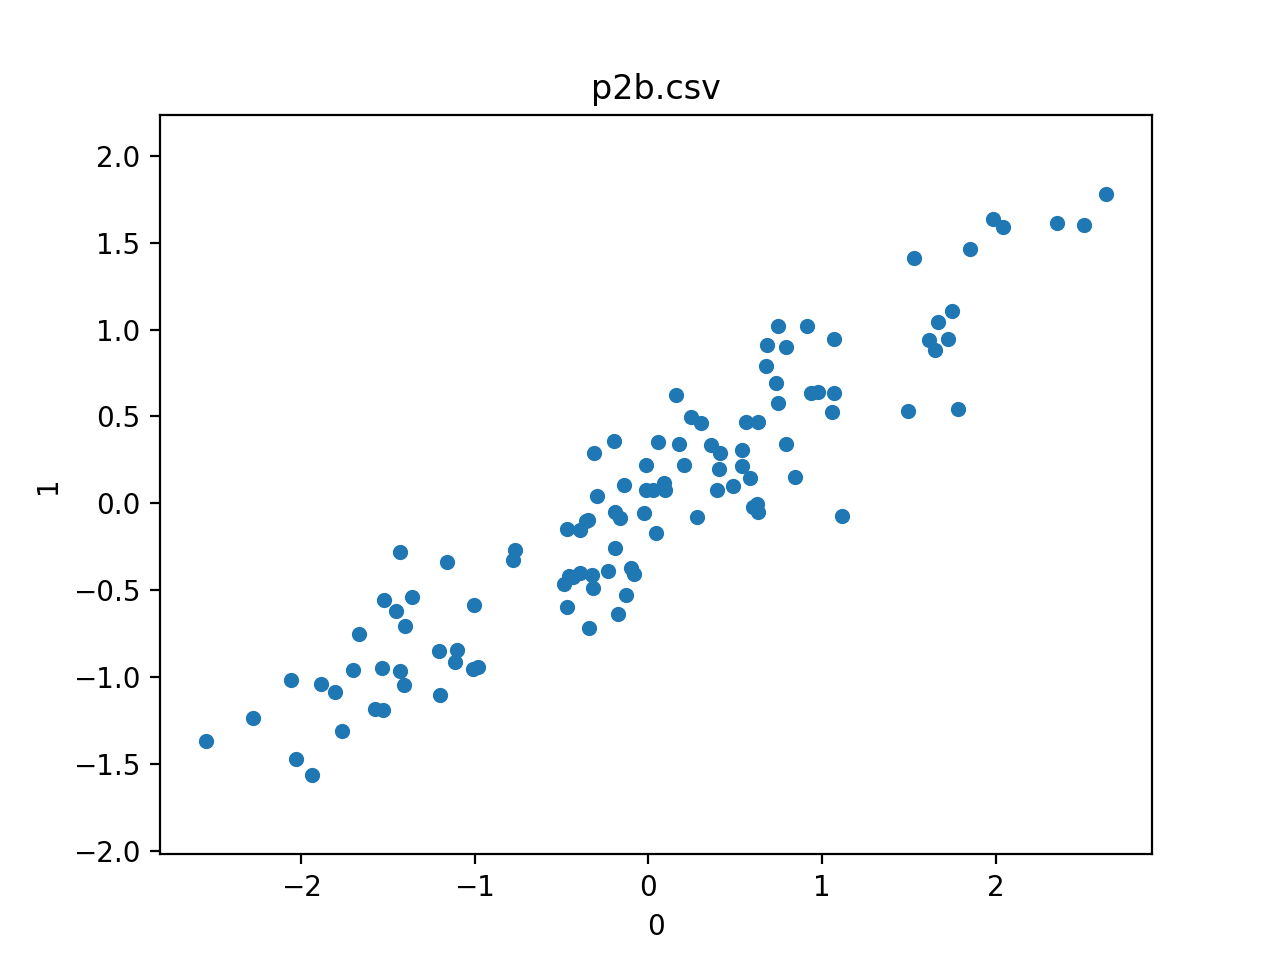
\includegraphics[width=\linewidth]{{fig/fig_p2b_1.png}}
\endminipage\hfill
\minipage{0.32\textwidth}%
  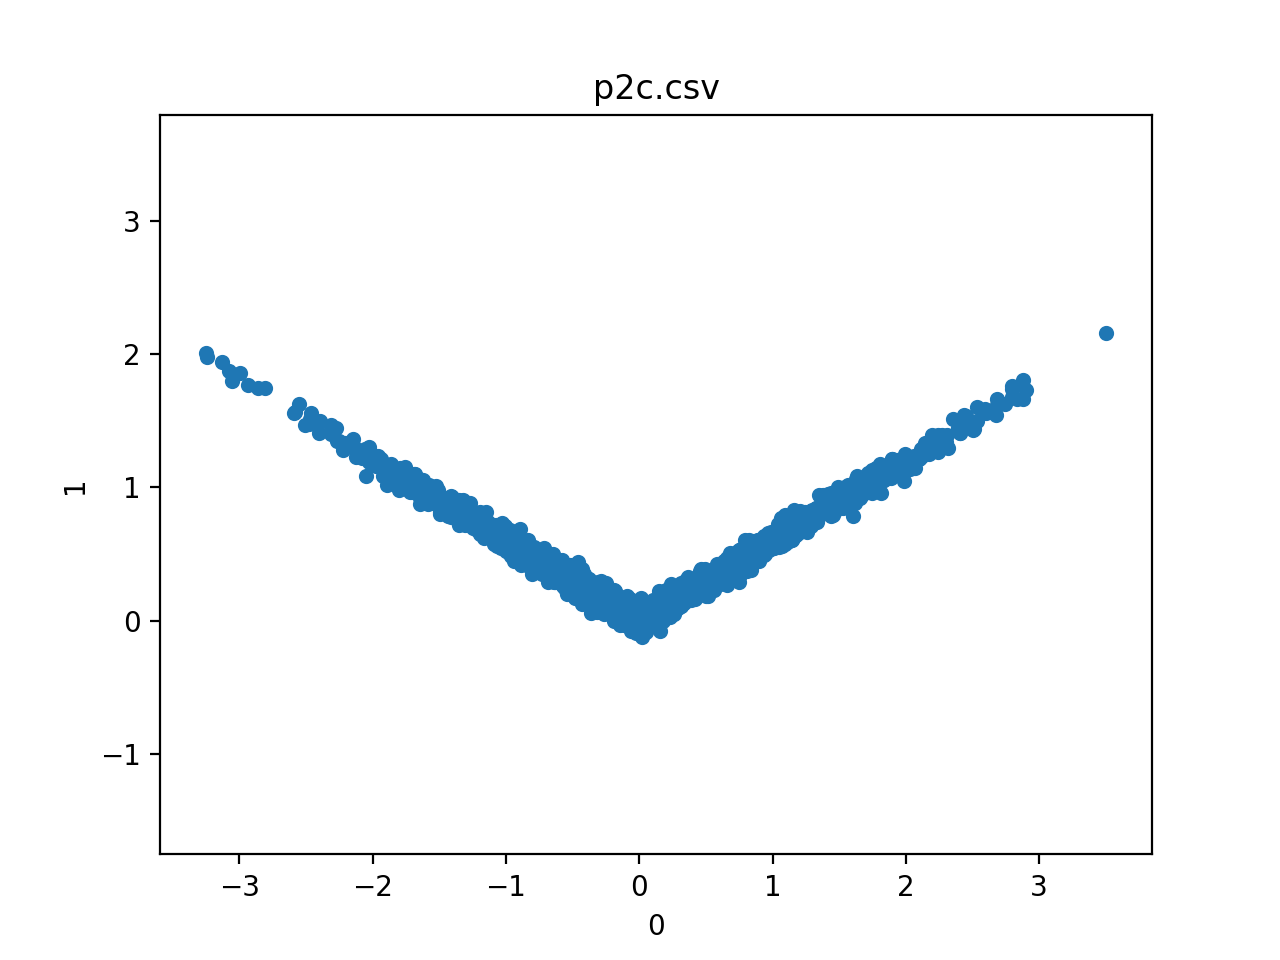
\includegraphics[width=\linewidth]{{fig/fig_p2c_1.png}}
\endminipage
\end{figure}

\subsection*{Part (a)}

By setting the $\alpha$ threshold to be $5\%$, there is a statistically significant association between the two variables in \ilc{p2a.csv} according to our findings. Since output we got are:



\noindent where the calculated p-value $p_a = 1.0409455130019734e-83$ is way lower than $0.05$, which means it is extremely unlikely to have an uncorrelated system to produce this kind of dataset by accident.\newline

In terms of the magnitutde and direction of the association, our finding suggests there isn't much as we have a $r_a = 0.38087503578373016$, which is not very high. However, we are able to tell that there is an association (between the two variables) in the positive direction, as we have an $r_a > 0$; and the magnitutde is rather medium as $r_a \not > 0.5$ -- which is about the right idea by inspecting the scatter plot of this dataset, where we almost have a circle centered around the \ilc{(0, 0)} oirgin; implying that for a random pair of data selected, there are roughly $\frac{1}{2}$ of the chance that the two data are deemed to be positively correlated.


\subsection*{Part (b)}

The output we got are:

\ilc{p2b.csv Corr: 0.9312196333264213; P-value: 3.7373210084392476e-49}

\noindent By setting the $\alpha$ threshold to be $5\%$, there is a statistically significant association between the two variables in \ilc{p2b.csv} according to our findings. Also as the value of $r_b$ is $> 0$ and very high, we may safetly conclude, base on our findings, that there is a positive association between the two variable with strong magnitutde.

To answer the asked questions, according to our findings:

\begin{itemize}
    \item \ilc{p2b.csv} has a stronger correlation coefficient.
    \item \ilc{p2a.csv} has a stronger p-value (``stronger'' in the sense of the dataset is less likely to be produced an uncorrelated system).
    \item No, the comparsions according to correlation coefficients and p-values do not agree on which pair indicates stronger association. We believe the decrepancy is due to first the two p-values are already extremely low, so ``having a slightly higher p-value'' shouldn't be an partical argument against the association found in \ilc{p2b.csv}. Second, by inspecting the scatter plots of \ilc{p2a.csv} and \ilc{p2b.csv}, we may tell that as the data showed in \ilc{p2b.csv} -- being almost linear -- is indeed more likely to be reproduced by an uncorrelated system (see demonstration\footnote{Source: SPSS Tutorials \textit{``Pearson Correlations -- Quick Introduction''} \url{https://www.spss-tutorials.com/pearson-correlation-coefficient/}} below). Also note it is my understanding that why $p_a < p_b$ is not a really important question to answer as $r_a$ is low already, so at best \ilc{p2a.csv} is ``a weakly associated dataset that can hardly be generated by an uncorrelated system'' -- this won't make \ilc{p2a.csv} having more association than an strongly correlated (with high $r_b$) \ilc{p2b.csv}.
    \item By inspecting the scatter plots we may clearly conclude that \ilc{p2b.csv} has a stronger association as a linear correlation is demonstrated. This observation is reflected on our findings as the high correlation coefficients implies correlation between two variables, and a low but slightly higher p-values is also interperable as we discussed above.
    \item Our conclusion with agree with the comparision of correlation coefficient, but not so much on p-values. This is, again, because both datasets have a extremely low p-value, so it is over-conservative to reject an associated hypothesis just because one of them is a bit higher. We may further reinforce the the finding by showing \ilc{p2b.csv} has a $95\%$ CI to be \ilc{[0.9010958855035053, 0.9523981653515785]}, (for reference, the $95\%$ CI for \ilc{p2a.csv} is \ilc{[0.3461386891983423, 0.41456855988502817]}) which does not include 0. So it is definately safe to claim correlation on \ilc{p2b.csv} and with the higher correlation coefficient and linear scatter plot, we may safetly conclude that \ilc{p2b.csv} has stronger association.
\end{itemize}

\begin{figure}[H]
    \centering
    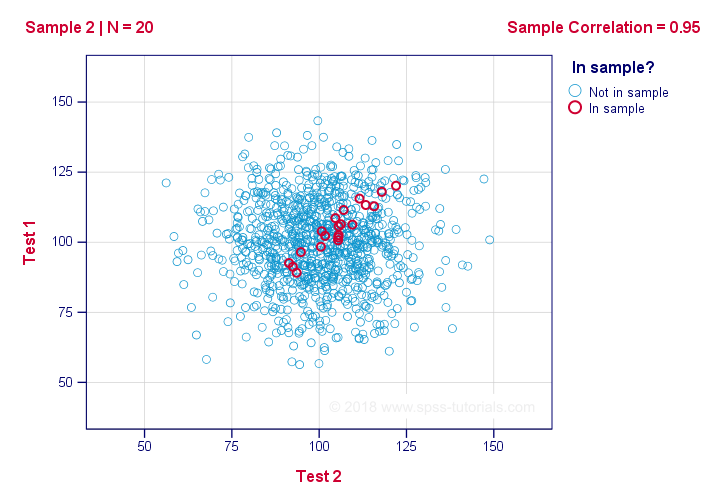
\includegraphics[width=0.7\linewidth]{{fig/fig_p2b.png}}
    \caption{Demonstration of the potential of finding a correlated dataset out of an uncorrelated system}
\end{figure}

\subsection*{Part (c)}

The output we got are:

\ilc{p2c.csv Corr: 0.04117899777683179; P-value: 0.05919591660545298}

\noindent By setting the $\alpha$ threshold to be $5\%$, there is \textbf{NOT} a statistically significant association between the two variables in \ilc{p2c.csv} according to our findings (as $p_c > 0.05$). Also although we have $r_c$ is $> 0$, indicating positive correlation, the value of $r_c$ is so low that we can't claim any correlation to a significant magnitutde.

To answer the asked questions, according to our findings:

\begin{itemize}
    \item \ilc{p2a.csv} has a stronger correlation coefficient.
    \item \ilc{p2a.csv} has a stronger p-value (``stronger'' in the sense of the dataset is less likely to be produced an uncorrelated system).
    \item Yes, the comparsions according to correlation coefficients and p-values do agree on which pair indicates stronger association.
    \item By inspecting the scatter plots we may clearly conclude that \ilc{p2c.csv} has a stronger association as a ``v-shape'' relationship is demonstrated. This is not reflected in the correlation coefficient and p-value because \textsc{Pearson's-R} coefficient has its drawbacks on dealing with dataset of nonlinear relationships (see demonstration\footnote{Source: Wikipedia \textit{``Pearson correlation coefficient''.} \url{https://en.wikipedia.org/wiki/Pearson_correlation_coefficient}} below, this is due to its relay on \ilc{Cov(x, y)}). The dataset we got in \ilc{p2c.csv} happen to be non-linear, thus the findings failed to reveal its association between two variables.
    \item Our conclusion does not agree with the comparision of correlation coefficients and p-values. This is due to the two findings cannot capture non-linear relationships -- which happen to be the case of \ilc{p2c.csv}.
\end{itemize}

\begin{figure}[H]
    \centering
    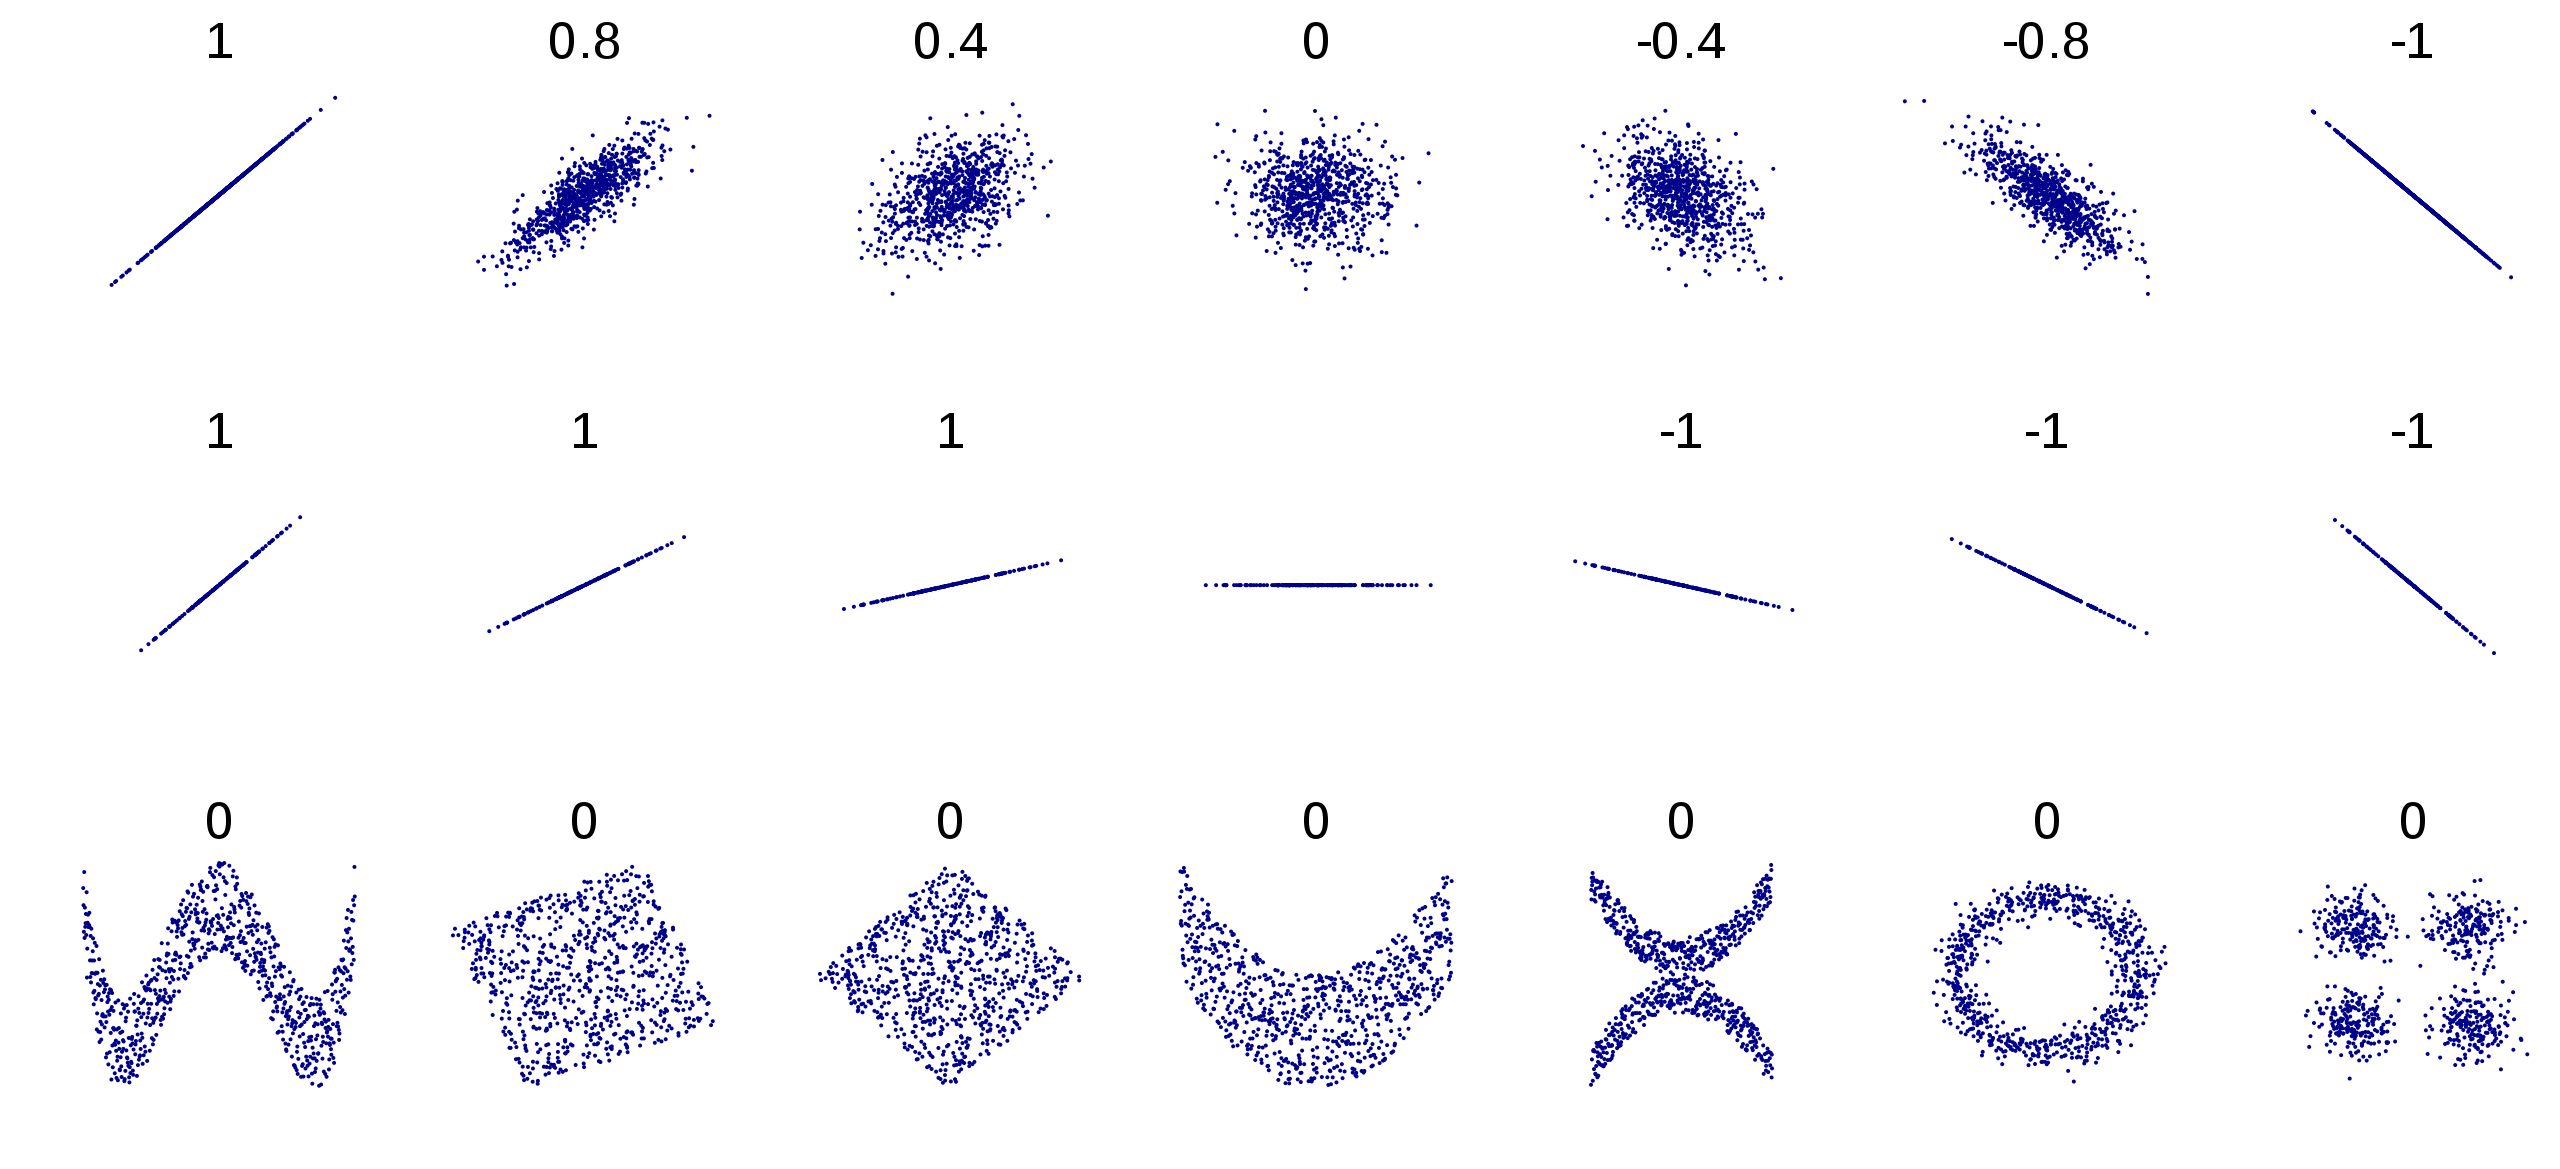
\includegraphics[width=1\linewidth]{{fig/fig_p2c.png}}
    \caption{Demonstration of correlation coefficient insensative to slope and non-linear relationship}
\end{figure}

\section*{Code}

Some of the script used in this assignment are rather long, please refer to \url{https://github.com/choH/csds313_written_assignments/tree/master/assignment_3/code} if you are interested to review.

\noindent (note we had some trouble with \textbf{Problem 1(b)}), the final version of code for that is \ilc{p1b\_alt.py}, thank you.)

\end{document}